% Options for packages loaded elsewhere
\PassOptionsToPackage{unicode}{hyperref}
\PassOptionsToPackage{hyphens}{url}
\PassOptionsToPackage{dvipsnames,svgnames*,x11names*}{xcolor}
%
\documentclass[
]{report}
\usepackage{lmodern}
\usepackage{amssymb,amsmath}
\usepackage{ifxetex,ifluatex}
\ifnum 0\ifxetex 1\fi\ifluatex 1\fi=0 % if pdftex
  \usepackage[T1]{fontenc}
  \usepackage[utf8]{inputenc}
  \usepackage{textcomp} % provide euro and other symbols
\else % if luatex or xetex
  \usepackage{unicode-math}
  \defaultfontfeatures{Scale=MatchLowercase}
  \defaultfontfeatures[\rmfamily]{Ligatures=TeX,Scale=1}
\fi
% Use upquote if available, for straight quotes in verbatim environments
\IfFileExists{upquote.sty}{\usepackage{upquote}}{}
\IfFileExists{microtype.sty}{% use microtype if available
  \usepackage[]{microtype}
  \UseMicrotypeSet[protrusion]{basicmath} % disable protrusion for tt fonts
}{}
\makeatletter
\@ifundefined{KOMAClassName}{% if non-KOMA class
  \IfFileExists{parskip.sty}{%
    \usepackage{parskip}
  }{% else
    \setlength{\parindent}{0pt}
    \setlength{\parskip}{6pt plus 2pt minus 1pt}}
}{% if KOMA class
  \KOMAoptions{parskip=half}}
\makeatother
\usepackage{xcolor}
\IfFileExists{xurl.sty}{\usepackage{xurl}}{} % add URL line breaks if available
\IfFileExists{bookmark.sty}{\usepackage{bookmark}}{\usepackage{hyperref}}
\hypersetup{
  pdftitle={OV\_Histotypes: Report of Statistical Findings},
  pdfauthor={Derek Chiu},
  colorlinks=true,
  linkcolor=Maroon,
  filecolor=Maroon,
  citecolor=Blue,
  urlcolor=Blue,
  pdfcreator={LaTeX via pandoc}}
\urlstyle{same} % disable monospaced font for URLs
\usepackage[margin=1in]{geometry}
\usepackage{longtable,booktabs}
% Correct order of tables after \paragraph or \subparagraph
\usepackage{etoolbox}
\makeatletter
\patchcmd\longtable{\par}{\if@noskipsec\mbox{}\fi\par}{}{}
\makeatother
% Allow footnotes in longtable head/foot
\IfFileExists{footnotehyper.sty}{\usepackage{footnotehyper}}{\usepackage{footnote}}
\makesavenoteenv{longtable}
\usepackage{graphicx}
\makeatletter
\def\maxwidth{\ifdim\Gin@nat@width>\linewidth\linewidth\else\Gin@nat@width\fi}
\def\maxheight{\ifdim\Gin@nat@height>\textheight\textheight\else\Gin@nat@height\fi}
\makeatother
% Scale images if necessary, so that they will not overflow the page
% margins by default, and it is still possible to overwrite the defaults
% using explicit options in \includegraphics[width, height, ...]{}
\setkeys{Gin}{width=\maxwidth,height=\maxheight,keepaspectratio}
% Set default figure placement to htbp
\makeatletter
\def\fps@figure{htbp}
\makeatother
\setlength{\emergencystretch}{3em} % prevent overfull lines
\providecommand{\tightlist}{%
  \setlength{\itemsep}{0pt}\setlength{\parskip}{0pt}}
\setcounter{secnumdepth}{5}
\usepackage{titlesec, blindtext, color}

\titleformat{\chapter}[display]
  {\Huge\bfseries}
  {}
  {0pt}
  {\thechapter.\ }

\titleformat{name=\chapter,numberless}[display]
  {\Huge\bfseries}
  {}
  {0pt}
  {}

\titlespacing*{\chapter}{0pt}{0pt}{40pt}

\renewcommand{\bibname}{References}
\usepackage[]{natbib}
\bibliographystyle{apalike}

\title{OV\_Histotypes: Report of Statistical Findings}
\author{Derek Chiu}
\date{2020-01-06}

\begin{document}
\maketitle

{
\hypersetup{linkcolor=}
\setcounter{tocdepth}{1}
\tableofcontents
}
\listoftables
\listoffigures
\hypertarget{preface}{%
\chapter*{Preface}\label{preface}}
\addcontentsline{toc}{chapter}{Preface}

This report of statistical findings describes the classification of ovarian cancer histotypes using data from NanoString CodeSets.

Marina Pavanello conducted the initial exploratory data analysis, Cathy Tang implemented class imbalance techniques, Derek Chiu conducted the normalization and statistical analysis, and Aline Talhouk lead the project.

\hypertarget{introduction}{%
\chapter{Introduction}\label{introduction}}

Ovarian cancer has five major histotypes: high-grade serous carcinoma (HGSC), low-grade serous carcinoma (LGSC), endometrioid carcinoma (ENOC), mucinous carcinoma (MUC), and clear cell carcinoma (CCOC). A common problem with classifying these histotypes is that there is a class imbalance issue. HGSC dominates the distribution, commonly accounting for 70\% of cases in many patient cohorts, while the other four histotypes are spread over the rest.

In the NanoString CodeSets, we also run into a problem with trying to find suitable control pools to normalize the gene expression. For prospective NanoString runs, the pools can be specifically chosen, but for retrospective runs, we have to utilize a combination of common samples and common genes as references for normalization.

The supervised learning is performed under a consensus framework: we consider various classification algorithms and use evaluation metrics to help making decisions of which methods to carry forward.

\hypertarget{methods}{%
\chapter{Methods}\label{methods}}

\begin{center}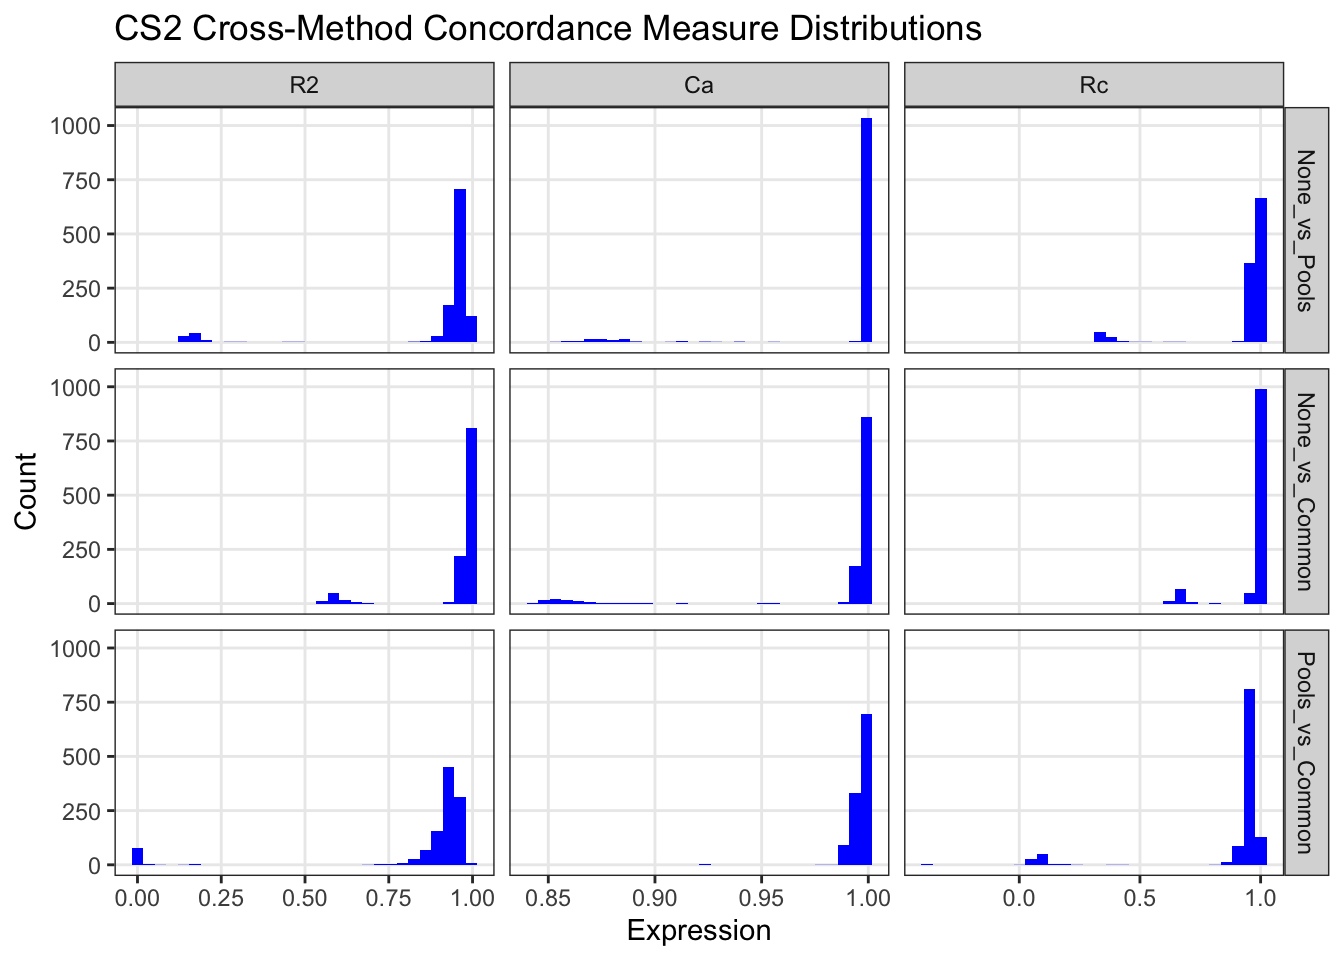
\includegraphics{OV_Histotypes_RSF_files/figure-latex/setup-02-1} \end{center}

\hypertarget{data-processing}{%
\section{Data Processing}\label{data-processing}}

There are 3 NanoString CodeSets:

\begin{itemize}
\tightlist
\item
  CS1: OvCa2103\_C953

  \begin{itemize}
  \tightlist
  \item
    Samples = 412
  \item
    Genes = 275
  \end{itemize}
\item
  CS2: PrOTYPE2\_v2\_C1645

  \begin{itemize}
  \tightlist
  \item
    Samples = 1223
  \item
    Genes = 384
  \end{itemize}
\item
  CS3: OTTA2014\_C2822

  \begin{itemize}
  \tightlist
  \item
    Samples = 5424
  \item
    Genes = 532
  \end{itemize}
\end{itemize}

These datasets contain raw counts extracted straight from NanoString RCC files.

\hypertarget{housekeeping-genes}{%
\section{Housekeeping Genes}\label{housekeeping-genes}}

The first normalization step is to normalize all endogenous genes to housekeeping genes (POLR1B, SDHA, PGK1, ACTB, RPL19; reference genes expressed in all cells). We normalize by subtracting the average log2 housekeeping gene expression from the log2 endogenous gene expression. The updated CodeSet dimensions are now:

\begin{itemize}
\tightlist
\item
  CS1: OvCa2103\_C953

  \begin{itemize}
  \tightlist
  \item
    Samples = 412
  \item
    Genes = 256
  \end{itemize}
\item
  CS2: PrOTYPE2\_v2\_C1645

  \begin{itemize}
  \tightlist
  \item
    Samples = 1223
  \item
    Genes = 365
  \end{itemize}
\item
  CS3: OTTA2014\_C2822

  \begin{itemize}
  \tightlist
  \item
    Samples = 5424
  \item
    Genes = 513
  \end{itemize}
\end{itemize}

The number of genes are reduced by 19: 5 housekeeping, 8 negative, 6 positive (the latter 2 types are not used).

\hypertarget{common-samples-and-genes}{%
\section{Common Samples and Genes}\label{common-samples-and-genes}}

Since the reference pool samples only exist in CS2 and CS3, we need to find an alternative method to normalize all three CodeSets. One method is to select common samples and common genes that exist in all three. We found 72 common genes. Using the \texttt{summaryID} identifer, we found 78 common summary IDs, which translated to 320 samples. The number of samples that were found in each CodeSet differed:

\begin{itemize}
\tightlist
\item
  CS1: OvCa2103\_C953

  \begin{itemize}
  \tightlist
  \item
    Samples = 93
  \item
    Genes = 72
  \end{itemize}
\item
  CS2: PrOTYPE2\_v2\_C1645

  \begin{itemize}
  \tightlist
  \item
    Samples = 87
  \item
    Genes = 72
  \end{itemize}
\item
  CS3: OTTA2014\_C2822

  \begin{itemize}
  \tightlist
  \item
    Samples = 140
  \item
    Genes = 72
  \end{itemize}
\end{itemize}

\hypertarget{cs1-training-set-generation}{%
\section{CS1 Training Set Generation}\label{cs1-training-set-generation}}

We use the reference method to normalize CS1 to CS3.

\begin{itemize}
\tightlist
\item
  CS1 reference set: duplicate samples from CS1

  \begin{itemize}
  \tightlist
  \item
    Samples = 25
  \item
    Genes = 72
  \end{itemize}
\item
  CS3 reference set: corresponding samples in CS3 also found in CS1 reference set

  \begin{itemize}
  \tightlist
  \item
    Samples = 20
  \item
    Genes = 72
  \end{itemize}
\item
  CS1 validation set: remaining CS1 samples with reference set removed

  \begin{itemize}
  \tightlist
  \item
    Samples = 387
  \item
    Genes = 72
  \end{itemize}
\end{itemize}

The final CS1 training set has 304 samples on 72 genes after normalization and keeping only the major histotypes of interest.

\hypertarget{cs2-training-set-generation}{%
\section{CS2 Training Set Generation}\label{cs2-training-set-generation}}

We use the pool method to normalize CS2 to CS3 so we can be consistent with the PrOTYPE normalization when there are available pools.

\begin{itemize}
\tightlist
\item
  CS3 pools:

  \begin{itemize}
  \tightlist
  \item
    Samples = 22
  \item
    Genes = 513
  \end{itemize}
\item
  CS2 pools:

  \begin{itemize}
  \tightlist
  \item
    Samples = 10
  \item
    Genes = 365
  \end{itemize}
\end{itemize}

The final CS2 training set has 945 samples on 136 (common) genes after normalization
and keeping ony the major histotypes of interest.

\hypertarget{results}{%
\chapter{Results}\label{results}}

  \bibliography{packages.bib}

\end{document}
